\documentclass[12pt,a4paper]{article}

% Paquetes básicos
\usepackage[x11names]{xcolor}
\usepackage[utf8]{inputenc}
\usepackage{mathtools, amssymb, amsthm}
\usepackage{changepage}
\usepackage{geometry}
\usepackage[colorlinks=true]{hyperref}
\usepackage{enumitem}
\usepackage{etoolbox}
\usepackage{graphicx}
\usepackage{setspace}
\usepackage{tcolorbox}
\tcbuselibrary{skins, breakable}
\usepackage{titlesec}
\usepackage{tikz} % core TikZ
\usetikzlibrary{matrix}

% Margins
%\geometry{left=3cm,right=3cm,top=2.5cm,bottom=2.5cm}

% Custom operators
\newcommand{\card}{\operatorname{card}}
\newcommand{\muae}{\overset{\mu-a.e.}{=}}

% Implication box setup
\tcbset{Implication-number/.style={
  enhanced,
  boxsep=2pt,
  colback=white,
  frame hidden,
  sharp corners,
  left=2pt, right=2pt, top=1pt, bottom=1pt,
  underlay={
    \draw[line width=0.5pt] (frame.south west) -- ([xshift=-133mm]frame.south east); % línea horizontal
    \draw[line width=0.5pt] ([xshift=-133mm]frame.north east) -- ([xshift=-133mm]frame.south east); % línea vertical
  }
}}

\tcbset{Implication-number-ds/.style={
  enhanced,
  boxsep=2pt,
  colback=white,
  frame hidden,
  sharp corners,
  left=2pt, right=2pt, top=1pt, bottom=1pt,
  underlay={
    \draw[line width=0.5pt] ([yshift=5mm]frame.south west) -- ([xshift=-133mm, yshift=5mm]frame.south east); % línea horizontal
    \draw[line width=0.5pt] ([xshift=-133mm, yshift=-3mm]frame.north east) -- ([xshift=-133mm, yshift=5mm]frame.south east); % línea vertical
  }
}}

\tcbset{Subset-contingency/.style={
  enhanced,
  boxsep=2pt,
  colback=white,
  frame hidden,
  sharp corners,
  left=2pt, right=2pt, top=1pt, bottom=1pt,
  underlay={
    \draw[line width=0.5pt] (frame.south west) -- ([xshift=-140mm]frame.south east); % línea horizontal
    \draw[line width=0.5pt] ([xshift=-140mm]frame.north east) -- ([xshift=-140mm]frame.south east); % línea vertical
  }
}}

\tcbset{Indent-subset-contingency/.style={
  enhanced,
  boxsep=2pt,
  colback=white,
  frame hidden,
  sharp corners,
  left=2pt, right=2pt, top=1pt, bottom=1pt,
  underlay={
    \draw[line width=0.5pt] (frame.south west) -- ([xshift=-140mm+0.07\textwidth]frame.south east); % línea horizontal
    \draw[line width=0.5pt] ([xshift=-140mm+0.07\textwidth]frame.north east) -- ([xshift=-140mm+0.07\textwidth]frame.south east); % línea vertical
  }
}}

% Useful commands
\renewcommand{\contentsname}{Contenidos}

\newcommand{\R}{\mathbb{R}}
\newcommand{\N}{\mathbb{N}}
\newcommand{\Z}{\mathbb{Z}}
\newcommand{\Q}{\mathbb{Q}}
\newcommand{\C}{\mathbb{C}}

\newcommand{\smallcup}{\mathop{\cup}\limits}
\newcommand{\smallcap}{\mathop{\cap}\limits}
\newcommand{\smallsum}{\mathop{\sum}\limits}
\newcommand{\smallprod}{\mathop{\prod}\limits}

\newcommand{\linf}[1]{\displaystyle{\mathop{\underline{\lim}}_{#1}}}
\newcommand{\mlim}[1]{\displaystyle{\lim_{#1}}}

%Integral de Lebesgue con patas
\newcommand{\lbint}{\mathop{\int_{\!\!\!\!\!|\!}^{\!|\!}}}

% TODO: añadir
\newcommand{\elep}[2]{\mathcal{L}_{#1}(#2)}

% ----- Custom counters and counter commands -----
% Custom counter hierarchy
\newcounter{unit}[section]
\newcounter{chapter}[unit]
\makeatletter
\@addtoreset{subsubsection}{chapter}
\makeatother

\renewcommand{\theunit}{\arabic{unit}}
\renewcommand{\thechapter}{\arabic{chapter}}
\renewcommand{\thesubsubsection}{\theunit.\thechapter.\arabic{subsubsection}}

% Custom content hierarchy behavior
\newcommand{\chapter}[1]{
    \refstepcounter{chapter}
    \subsection*{\Large{\S \thechapter. #1}}
    \addcontentsline{toc}{subsection}{\thechapter. #1}
}
\newcommand{\unit}[1]{
    \refstepcounter{unit}
    \section*{\Huge{\Roman{unit} #1}}
    \addcontentsline{toc}{section}{\Roman{unit} #1}
}

\newcommand{\result}[1]{%
  \subsubsection{#1}%
  \label{result:\thesubsubsection}
}
  
\titleformat{\subsubsection}
    {\normalfont\large\bfseries} % mismo tamaño que \subsection
    {\thesubsubsection}{1em}{}
  
%---- Custom proof commands-----
\newcommand{\dem}{
    \noindent \underline{\textbf{Demostración:}}
}
\newcommand{\nota}{
    \noindent \underline{\textbf{Nota:}}
}
% ----------------------------------------
\hbadness=10000
\vbadness=10000
\hfuzz=100pt
\vfuzz=100pt
%------------------------------
\title{Análisis Matemático III}
\author{Javier Ortín Rodenas}
\date{Curso 2025-2026}

\begin{document}

\maketitle
\newpage
\hypersetup{linkcolor=black}
\tableofcontents
\hypersetup{linkcolor=Ivory4}
\newpage
\setcounter{unit}{2}
\unit{Espacios \texorpdfstring{$L_p$}{Lp} con \texorpdfstring{$1 \leq p \leq \infty$}{1 <= p <= infty}}
\hspace{3mm} A lo largo de esta unidad, consideraremos $(X, \Sigma, \mu)$ como un espacio de medida genérico.
\chapter{Primeras definiciones}
\vspace{2mm} \result{Definición de \texorpdfstring{$\mathcal{L}_p$}{Lp}}
\hspace{3mm} Para $1 \leq p < \infty$, denotaremos como $\mathcal{L}_p(X)$ o como $\mathcal{L}_p(X, \Sigma, \mu)$ al conjunto de funciones medibles $f : X \longrightarrow \R$ para las que se cumple
$$\int_{X}|f|^p\,d\mu < \infty$$
Asociada a cada $f \in \mathcal{L}_p(X)$, tenemos la siguiente cantidad numérica:
$$||f||_p := \left(\int_{X}|f|^p\,d\mu\right)^{\frac{1}{p}} $$
Nótese que para el caso $p = 1$ se corresponde con la \hyperref[result:2.2.3]{definición ya estudiada}.

\vspace{6mm}
\result{Definición de \texorpdfstring{$\mathcal{L}_\infty$}{L\_infty}}
\hspace{3mm} Para $p=\infty$, $\mathcal{L}_\infty(X) = \mathcal{L}_\infty(X, \Sigma, \mu)$ denota el conjunto de todas las funciones medibles $f : X \longrightarrow \R$ para las que existe $\alpha \in [0, +\infty)$ que verifica:
$$\mu\Big(\{x \in X : |f(x)| > \alpha \}\Big) = 0$$
Esta condición equivale a su vez a las dos siguientes:
\begin{align*}
    \mu\Big(X \setminus \{x \in X : |f(x)| \leq \alpha\} \Big) = 0 &&
    \{x \in X : |f(x)| \leq \alpha\} \overset{\mu-a.e.}{=} X
\end{align*}

\vspace{6mm}
\result{Funciones sumables y funciones de \texorpdfstring{$\mathcal{L}_p(X)$}{Lp(X)}}
\hspace{3mm} Si $f : X \longrightarrow \overline{\R}$ es medible, y $\int_{X}|f|^p\,d\mu < \infty$ (para $p < \infty$). Entonces, existe una función $g \in \mathcal{L}_p(X)$  tal que $f \overset{\mu-a.e.}{=} g$. Como consecuencia, si $p < \infty$,
$$\left(\int_{X}|f|^p\,d\mu\right)^\frac{1}{p} = ||g||_p $$
\vspace{2mm} \dem Extendemos lo visto en el \hyperref[result:2.2.6]{resultado 2.2.6}.
\vspace{2mm} \newline \indent Definimos los siguientes conjuntos auxiliares: \\[-4ex]
\begin{align*}
    A = \{x \in X : f(x) = +\infty\} && B = \{x \in X : f(x) = -\infty\}
\end{align*}
Ambos conjuntos han de ser de medida nula, o de lo contrario $\int_{X}|f|^p\,d\mu = \infty$. Así, basta considerar la siguiente función:
\begin{flalign*}
    g(x) = f(x) \cdot X_{X \setminus (A \cup B)}(x) =
    \begin{cases}
        f(x) &\text{si }x \notin A \cup B \\
        0 &\text{si } x \in A \cup B
    \end{cases}
\end{flalign*}
Como $\mu(A) = \mu(B) = 0$, tenemos que $f \overset{\mu-a.e.}{=} g$.

\vspace{6mm}
\result{Definición de supremo esencial}
\hspace{3mm} Para cada $f \in \mathcal{L}_\infty(X)$ definimos el siguiente conjunto:
$$A_f := \Big\{\alpha \in [0,\infty) : \mu\big(\{x \in X : f(x) > \alpha\}\big) = 0 \Big\} $$
A partir de él, definimos $||f||_p := \inf A_f$. Esta cantidad recibe el nombre de ``supremo esencial''.

\vspace{6mm}
\result{Mínimo esencial}
\hspace{3mm} El supremo esencial es en realidad un mínimo. Es decir; sea $f \in \mathcal{L}_\infty(X)$, se cumple:
$$||f||_\infty \in \Big\{f(x) : x \in X\}  \text{ o equivalentemente } ||f||_\infty = \min A_f$$
\dem \newline \vspace{2mm} Denotemos $\beta := \inf A_f$. Consideramos $(\beta_n)_{n\in\N} \subseteq A_f$ sucesión decreciente que verifica $\lim_{n\to\infty} \beta_n = \beta$. Para cada $n \in\N$ definimos el siguiente conjunto auxiliar:
$$B_n := \Big\{x \in X : |f(x)| \leq \beta_n \Big\}$$
\indent De este modo,  $\forall n \in \N$, $B_{n+1} \subseteq B_n$ y $B_n \in \Sigma$. Además, por ser $f \in \mathcal{L}_\infty(X)$ por hipótesis, tenemos que $B_n = X \setminus M_n$ con $M_n \in \Sigma$ tal que $\mu(M_n) = 0$. Por tanto, se cumple: \\[-3ex]
$$\{x \in X : |f(x)| \leq \beta\} = \smallcap_{n\in\N} B_n = \smallcap_ {n\in \N}(X \setminus M_n) = X \setminus (\smallcup_{n\in\N}M_n)$$
Por subaditividad, $\mu\big(\smallcup_{n\in\N} M_n\big) = 0$, luego $\beta \in A_f$ por definición.

\newpage
\chapter{Estructura de los \texorpdfstring{$\mathcal{L}_p$}{L\_p}}
\result{Concepto de convexidad}
\hspace{3mm} Una combinación convexa de puntos de un espacio afín es aquella combinación lineal de los mismos cuyos pesos sean no negativos y sumen $1$. Para el caso de dos puntos, $a$ y $b$, podemos expresar su combinación convexa como:
\begin{align*}
    \lambda a + (1-\lambda) b && \text{ con } \lambda \in [0,1]
\end{align*}
Nótese que conforme $\lambda$ va aumentando, se recorre el segmento en línea recta desde $a$ hasta $b$.
\vspace{4mm}\newline \indent Sea $A$ un conjunto de un espacio afín, diremos que es convexo si dados $a, b \in A$, tenemos que cualquier combinación conexa de ambos está también en $A$. Es decir,
$$A \text{ es convexo } \iff \hspace{2mm}\forall \hspace{1mm} a,b \in A, \hspace{2mm} \forall \hspace{1mm}\lambda \in [0,1] : \lambda a + (1-\lambda) b \in A  $$
Intuitivamente, se corresponde con que todo segmento que une dos puntos de $A$ está contenido al completo en $A$.
\\[3ex]
\begin{minipage}{0.5\textwidth}
    \begin{center}
        \def\p{0.3}
        \def\delt{0.75}
        \begin{tikzpicture}[scale=2]
            \filldraw[HotPink2!40, thick]
            plot[domain=0:360, samples=400] 
            ({ sign(cos(\x)) * abs(cos(\x))^(1/\p) },
            { sign(sin(\x)) * abs(sin(\x))^(1/\p) });
            \filldraw[black] (-\delt,0) circle (0.5pt);
            \filldraw[black] (0,\delt) circle (0.5pt);
            \draw[-] (-\delt, 0) -- (0,\delt);
        \end{tikzpicture}
        
        \noindent Conjunto no convexo
    \end{center}
\end{minipage}
\begin{minipage}{0.5\textwidth}
    \begin{center}
        \def\p{0.3}
        \def\delt{0.75}
        \begin{tikzpicture}[scale=2]
            \filldraw[DarkSeaGreen2!40, thick]
            plot[domain=0:360, samples=400] 
            ({cos(\x)},{sin(\x)});
            \filldraw[black] (-\delt,0) circle (0.5pt);
            \filldraw[black] (0,\delt) circle (0.5pt);
            \draw[-] (-\delt, 0) -- (0,\delt);
        \end{tikzpicture}
        
        \noindent Conjunto convexo
    \end{center}
\end{minipage}

\vspace{9ex} Veamos ahora cómo se traduce este concepto a funciones.
\newpage Diremos que una función $f : \R \longrightarrow \R$ es convexa en un intervalo $I$ si el segmento que une dos puntos cualesquiera de su grafo en $I$ queda por encima del propio grafo. Es decir, si verifica:
$$\forall x_1, x_2 \in I : f\big(\lambda x_1 + (1-\lambda)x_2\big) < \lambda f(x_1) + (1-\lambda)f(x_2) \hspace{6mm} \forall \lambda \in [0,1]$$
Esto a su vez equivale a exigir que el siguiente conjunto (epigrafo de $f$) sea convexo:
$$\{(x,y) : x \in I, y > f(x)\} $$
Podemos extender la definición de convexidad de funciones al estudiar conjuntos convexos más generales y no solo intervalos.

\begin{center}
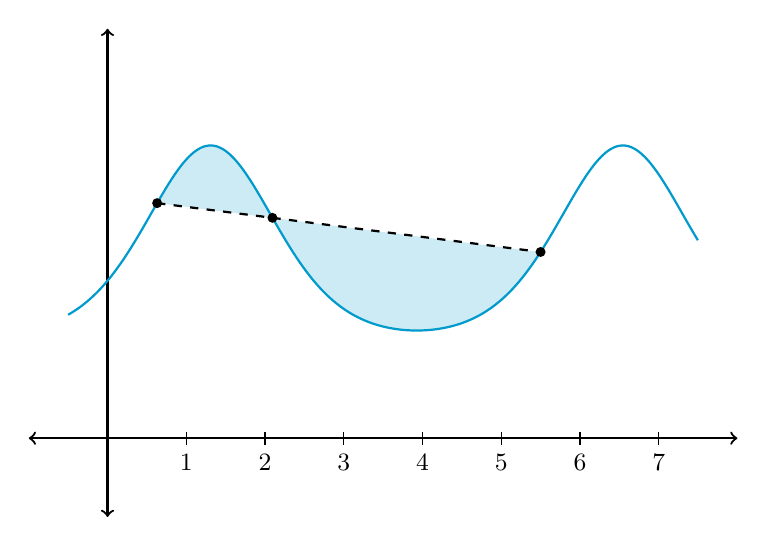
\begin{tikzpicture}
    % interval
    \def\xstart{0.63}
    \def\xend{5.5}
    \pgfmathdeclarefunction{f}{1}{%
    \pgfmathparse{1 + exp(sin(1.2 * #1 r))}%
    }
    \pgfmathparse{f(\xstart)} \let\fstart\pgfmathresult
    \pgfmathparse{f(\xend)}   \let\fend\pgfmathresult
    \pgfmathsetmacro{\m}{(\fend-\fstart)/(\xend-\xstart)}
    % (optional) declare g(x) if you want to call it
    \pgfmathdeclarefunction{g}{1}{%
    \pgfmathparse{\m*(#1-\xstart) + \fstart}%
    }

    \def\maxX{7}
    \def\maxY{5}
    \draw[<->, thick] (-1,0) -- (\maxX+1,0);
    \draw[<->, thick] (0,-1) -- (0,\maxY+0.2);
    \foreach \i in {1,...,7} {
    \draw (\i,0.08) -- (\i,-0.08) node[below] {\small $\i$};
    }
    \fill[DeepSkyBlue3!20] 
    (\xstart,\fstart)
    plot[domain=\xstart:\xend, samples=240, smooth] (\x,{f(\x)})
    -- (\xstart,\fstart) -- cycle;

    \draw[thick, DeepSkyBlue3] 
    plot[domain=-0.5:\maxX+0.5, samples=600, smooth] (\x,{f(\x)});
    %Bounding line
    \draw[dashed, thick] (\xstart,\fstart) -- (\xend,\fend);

    \foreach \i in {0.63, 2.09484, 5.5} {
      \fill (\i,{f(\i)}) circle (1.8pt);
    }

\end{tikzpicture}

\noindent La función no es convexa en $[0,6]$, pero sí en $[2,6]$.
\end{center}

\vspace{4mm} Podemos considerar definiciones distintas de convexidad según exijamos o no que la desigualdad sea estricta.

\vspace{6mm}
\result{Los \texorpdfstring{$\mathcal{L}_p(X)$}{L\_p(X)} son espacios vectoriales}
\hspace{3mm} Para $1 \leq p \leq \infty$, $\mathcal{L}_p(X)$ es un espacio vectorial.
\vspace{6mm} \newline \dem Distinguiremos varios casos:
\vspace{2mm} \newline \noindent $\bullet$ Caso $p=1$: \hyperref[result:2.2.4]{ya se ha demostrado}.
\vspace{2mm} \newline \noindent $\bullet$ Caso $p= \infty$:
\begin{adjustwidth}{0.07\textwidth}{}
    \vspace{-4mm} Sea $f \in \mathcal{L}_\infty(X)$, sea $\lambda \in \R$. Veamos $\lambda f \in \mathcal{L}_\infty(X)$.
    \vspace{2mm} \newline Si $\lambda = 0$, $\lambda f \equiv 0 \in \mathcal{L}_\infty(X)$.
    \vspace{2mm} \newline Sea $\lambda \in \R \setminus \{0\}$. Como $f \in \mathcal{L}_\infty(X)$, $\exists$ $M \in \Sigma$ con $\mu(M) = 0$ tal que:
    $$X \setminus M = \{x \in X : |f(x)|\leq ||f||_\infty\} = \{x \in X : |\lambda f(x)|\leq |\lambda|\cdot ||f||_\infty\}$$
    Tenemos que $\lambda f \in \mathcal{L}_\infty(X)$ por definición.

    \vspace{5mm} Sean $f,g\in \elep{\infty}{X}$, veamos que $f+g\in \elep{\infty}{X}$:
    \vspace{2mm} \newline Por definición, $\exists \hspace{1mm} M,N \in \Sigma$ con $\mu(M) = \mu(N) = 0$ tales que: \\[-3ex]
    \begin{align*}
        X \setminus M = \{x \in X : |f(x)| \leq ||f||_\infty\} &&
        X \setminus N = \{x \in X : |g(x)| \leq ||g||_\infty\} 
    \end{align*}
    Entonces, dado $x \in X \setminus(M \cup N)$ cualquiera, se cumple:
    $$|f(x) + g(x) | \leq |f(x)| + |g(x)| \leq ||f||_{\infty} + ||g||_{\infty} < \infty $$
    Como $\mu(M \cup N) = 0$, tenemos $f+g\in \elep{\infty}{X}$ por definición.
\end{adjustwidth}
\vspace{6mm} \noindent $\bullet$ Caso $1 < p < \infty$:
\begin{adjustwidth}{0.07\textwidth}{}
    Sean $\lambda \in \R, f \in \elep{p}{X}$. Veamos que $\lambda f \in \elep{\infty}{X}$.
    $$\int_{X}|\lambda f(x)|^p\,d\mu(x) = |\lambda|^p \cdot \int_{X}|f(x)|^p\,d\mu(x) = |\lambda|^p \cdot ||f||_p^p < \infty$$
    Se cumple por definición.

    \vspace{4mm} Sean $f,g \in \elep{p}{X}$. Veamos que $f+g\in \elep{p}{X}$:
    \begin{flalign*}
        \int_{X}&|f(x)+p(x)|\,d\mu(x) = \int_{X} \Big|\hspace{1mm} \underbrace{\frac{1}{2}}_\lambda\cdot 2 \cdot f(x)+ \underbrace{\frac{1}{2}}_{1-\lambda}\cdot 2 \cdot g(x)\hspace{1mm} \Big|^p\,d\mu(x) = (*)
    \end{flalign*}
    La función $h(t) = |t|^p$ es convexa en $[0,+\infty]$ para $p > 1$. Por tanto,
    \begin{flalign*}
        (*) &\leq \int_{X}\frac{1}{2}\left|2f(x)\right|^p + \frac{1}{2} |2g(x)|^p\,d\mu(x) = 2^{p-1}\cdot \int_{X}|f(x)|^p\,d\mu(x) + 2^{p-1} \cdot \int_{X}|g(x)|^{p}\,d\mu(x) = &&\\
        &= 2^{p-1}\left(\int_{X}|f(x)|^p\,d\mu(x) + \int_{X}|g(x)|^p\,d\mu\right) = 2^{p-1}\big(||f||_p^p + ||g||_p^p\big) < \infty
    \end{flalign*}
    Se cumple por definición.
\end{adjustwidth}

\vspace{6mm}
\result{Conjugado \texorpdfstring{$p^*$}{p*}}
\hspace{3mm} Para cada $p \in [1, +\infty]$, denotaremos como $p^*$ al único número en $\overline{\R}$ que verifica:
$$\frac{1}{p} + \frac{1}{p^*} = 1$$
Solo hay un único número en todo $\overline{\R}$ que verifica esto, pero ha de estar necesariamente en $(1, \infty)$:
$$\frac{1}{p} + \frac{1}{p^*} = 1 \Rightarrow p^* = \frac{1}{1 - \frac{1}{p}} = \frac{p}{p-1} \overset{p\in[1,\infty]}{\in} (1, \infty)$$
\indent Estas son algunas de las propiedades de este conjugado (claras por la definición):
\begin{align*}
    (p^*)^* = p && p + p^* = p\cdot p^* && p\cdot p^* - p^*p && p^* = \frac{p}{p-1} && p^*(p-1) = p
\end{align*}

\vspace{6mm}
\result{Desigualdad de Hölder}
\hspace{3mm} Sean $f \in \elep{p}{X}$, $g \in \elep{p^*}{X}$. Entonces, se cumple:
\begin{align*}
    f\cdot g \in \elep{1}{X} && ||f\cdot g||_1 \leq ||f||_p \cdot ||g||_{p^*}
\end{align*}
\vspace{3mm} \dem
\vspace{2mm} \newline $\bullet$ Caso $p = 1, p^* = \infty$:
\begin{adjustwidth}{0.07\textwidth}{}
    \vspace{2mm} Como $g \in \elep{\infty}{X}$, $\exists$ $M \in \Sigma$ con $\mu(M) = 0$ tal que
    $$X \setminus M = \{x \in X : |g(x)| \leq ||g||_\infty\}$$
    Por tanto, ha de cumplirse:
    \begin{flalign*}
      \int_{X}&=|f\cdot g|\,d\mu = \int_{X \setminus M}|f(x)| \cdot |g(x)|\,d\mu(x) \leq \int_{X \setminus M}|f(x)| \cdot ||g||_\infty\,d\mu = &&\\
      &= ||g||_\infty \cdot \int_{X \setminus M}|f(x)|\,d\mu(x) = ||g||_\infty \cdot ||f||_1 < \infty
    \end{flalign*}
    Se cumple por definición.    
\end{adjustwidth}

\vspace{6mm} \noindent $\bullet$ Caso $1 < p < \infty$. Hay que estudiar dos posibles escenarios:
\vspace{2mm} \newline \indent a) Si $||f||_p = 0$ ó $||g||_{p^*} = 0$ (pudiendo darse ambas). Supongamos sin pérdida de generalidad que $||f||_p = 0$:
\newpage
\begin{adjustwidth}{0.07\textwidth}{}
    \vspace{2mm} $||f||_p = 0 \Rightarrow = \int_{X}|f|^p\,d\mu(x) = 0 \overset{\hyperref[result:2.1.17]{2.1.17}}{\Rightarrow} |f|^p \muae 0 \Rightarrow f \muae 0$.
    \vspace{2mm} \newline De este modo, $f \cdot g \muae 0 \Rightarrow |f\cdot g| = 0 \overset{\hyperref[result:2.1.17]{2.1.17}}{\Rightarrow} 0 = \int_{X}\,|f\cdot g|d\mu = ||f\cdot g||_1$.
\end{adjustwidth}

\vspace{6mm} b) \noindent Supongamos ahora que $||f||_p \neq 0 \neq ||g||_{p^*}$. Así,
\begin{adjustwidth}{0.07\textwidth}{}
    \vspace{3mm} Definimos los siguientes conjuntos auxiliares: \\[-3ex]
    \begin{align*}
        A := \{x \in X : f(x) = 0\} \in \Sigma &&  B := \{x \in X : g(X) = 0\} \in \Sigma
    \end{align*}
    Por cómo los hemos definido,
    $$\int_{X}\frac{|f(x)|}{||f||_p}\cdot \frac{|g(x)|}{||g||_{p^*}}\,d\mu(x) = \int_{X \setminus(A\cup B)}\frac{|f(x)|}{||f||_p} \cdot \frac{|g(x)|}{||g||_{p^*}}\,d\mu(x) = (*_1)$$
    Al tratarse de cantidades positivas, para cada $x \in X \setminus (A\cup B)$, existen $\xi_x, \zeta_x \in (0, \infty)$ tales que:
    \begin{align*}
      \frac{|f(x)|}{||f||_p} = e^{\frac{\xi_x}{p}} = \exp\left(\frac{\xi_x}{p}\right) &&\frac{|g(x)|}{||g||_{p^*}} = e^{\frac{\zeta_x}{p^*}} = \exp\left(\frac{\zeta_x}{p^*}\right)
    \end{align*}
    Sustituyendo en la expresión anterior:
    \begin{flalign*}
        (*_1) = \int_{X \setminus (A\cup B)}\hspace{-3mm} \exp\left(\frac{\xi_x}{p}\right) \cdot \exp\left(\frac{\zeta_x}{p^*}\right)\,d\mu(x) = \int_{X \setminus(A \cup B)}\hspace{-3mm} \exp\left(\frac{1}{p}\xi_x + \frac{1}{p^*}\zeta_x\right)\,d\mu(x)
    \end{flalign*}
    La función exponencial es convexa. Tomando $\lambda = \frac{1}{p}$, $1-\lambda = \frac{1}{p^*}$, tenemos:
    \begin{flalign*}
        (*_1) \leq \hspace{-3mm} \mathop{\int}_{X\setminus(A\cup B)}\hspace{-3mm} \frac{1}{p}\exp(\xi_x) + \frac{1}{p^*}\exp(\zeta_x)\,d\mu(x) = \frac{1}{p} \hspace{-5mm} \mathop{\int}_{X \setminus(A \cup B)}\hspace{-5mm} \exp(\xi_x)\,d\mu(x) + \frac{1}{p^*} \hspace{-5mm} \mathop{\int}_{X \setminus (A\cup B)}\hspace{-5mm} \exp(\zeta_x)\,d\mu(x) = (*_2)
    \end{flalign*}
    Deshacemos el cambio de variable y comparamos con la definición de $||\cdot||_p$ y de $||\cdot||_{p^*}$,
    \begin{flalign*}
        (*_2) &= \frac{1}{p} \hspace{-5mm}\mathop{\int}_{X \setminus(A\cup B)}\hspace{-3mm} \frac{|f(x)|^p}{||f||_p^p}\,d\mu(x) + \frac{1}{p^*} \hspace{-5mm} \mathop{\int}_{X \setminus(A \cup B)}\hspace{-3mm} \frac{|g(x)|^{p^*}}{||g||^{p^*}_{p^*}}\,d\mu(x) \leq &&\\
        &\leq \frac{1}{p \cdot ||f||^p_p} \cdot {\int}_{X}|f(x)|^p\,d\mu(x) + \frac{1}{p^* \cdot ||g||^{p^*}_{p^*}} \cdot {\int}_{X} \hspace{2mm} |g(x)|^{p^*}\,d\mu(x) = \\
        &= \frac{1}{p \cdot ||f||^p_p} \cdot ||f||^p_p + \frac{1}{p^* \cdot ||g||^{p^*}_{p^*}} \cdot ||g||^{p^*}_{p^*} = \frac{1}{p} + \frac{1}{p^*} = 1
    \end{flalign*}
    \newpage \noindent Sustituimos para resolver el problema inicial:
    \begin{flalign*}
        \int_{X}\frac{|f(x)|}{||f||_p}\cdot \frac{|g(x)|}{||g||_{p^*}}\,d\mu(x)
        \Rightarrow \int_{X}|f(x) \cdot g(x)|\,d\mu(x) \leq ||f||_p \cdot ||g||_{p^*} < \infty
    \end{flalign*}
\end{adjustwidth}

\vspace{6mm} \result{Desigualdad de Minkowski}
\hspace{3mm} Sea $1 \leq p \leq \infty$. Sean $f,g \in \elep{p}{X}$. Entonces, $||f+g||p \leq ||f||_p + ||g||_p$.
\vspace{4mm} \newline \dem Hemos de distinguir tres casos.
\vspace{2mm} \newline $\bullet$ Caso $p=1$: \hyperref[result:2.1.9]{ya ha sido probado}.
\vspace{2mm} \newline $\bullet$ Caso $p=\infty$:
\begin{adjustwidth}{0.07\textwidth}{}
    \vspace{2mm} Por ser $f,g \in \elep{\infty}{X}$, sabemos $\exists$ $M,N \in \Sigma$ con $\mu(M) = \mu(N) = 0$ tales que: \\[-3ex]
    \begin{align*}
        X \setminus M = \{x \in X : |f(x)| \leq ||f||_\infty\} && X \setminus N = \{x \in X : |g(x)| \leq ||g||_\infty\}
    \end{align*}
    Entonces, dado $x \in X \setminus (M \cup N)$, se cumple:
    $$|f(x) + g(x)| \leq |f(x)| + |g(x)| \leq ||f||_\infty + ||g||_\infty $$
    Como $\mu(M\cup N) = 0$. Recordando la (\hyperref[result:3.1.4]{notación 3.1.4}), tenemos:
    $$||f||_\infty + ||g||_\infty \in A_{f+g} \Rightarrow ||f+g||_\infty = \min A_{f+g} \leq ||f||_\infty + ||g||_\infty$$
\end{adjustwidth}
\vspace{4mm} $\bullet$ Caso $1 < p < \infty$:
\begin{adjustwidth}{0.07\textwidth}{}
    \vspace{-4ex}
    \begin{flalign*}
        &||f+p||_p^p = \int_{X}|f+g|^p\,d\mu = \int_{X}|f+g| \cdot |f+g|^{p-1}\,d\mu \leq &&\\[2ex]
        &= \hspace{2mm} \int_{X}\underbracket{\hspace{0.5mm} |f| \hspace{0.5mm}}_{\elep{p}{X}} \cdot \underbracket{\hspace{0.5mm}|f+g|^{p-1} \hspace{0.5mm}}_{\elep{p^*}{X}}\,d\mu
            + \int_{X}\underbracket{\hspace{0.5mm} |g| \hspace{0.5mm}}_{\elep{p}{X}} \cdot \underbracket{\hspace{0.5mm}|f+g|^{p-1} \hspace{0.5mm}}_{\elep{p^*}{X}}\,d\mu = (*)
    \end{flalign*}
    Por las \hyperref[result:3.2.3]{propiedades de $p^*$}, tenemos que:
    $$\int_{X}\left(|f + g|^{p-1}\right)^{p^*}\,d\mu = \int_{X}|f + g|^{p^*(p-1)}\,d\mu = \int_{X}|f+g|^p\,d\mu = ||f+g||_p^p < \infty$$
    Podemos aplicar la \hyperref[result:3.2.4]{Desigualdad de Hölder} a ambos sumandos: \newpage
    \begin{flalign*}
        (*) &\leq ||f||_p \cdot \Big| \Big| |f+g|^{p-1} \Big| \Big{|}_{p^*} + ||g||_p \cdot \Big| \Big| |f+g|^{p-1} \Big| \Big{|}_{p^*} = (||f||_p + ||g||_p) \cdot \Big| \Big| |f+g|^{p-1} \Big| \Big{|}_{p^*} = &&\\[2ex]
        &= (||f||_p + ||g||_p) \cdot \left(\int_{X}|f+g|^{p^*(p-1)}\,d\mu\right)^\frac{1}{p^*} = (||f||_p + ||g||_p) \cdot \left(||f+g||_p^p\right)^\frac{1}{p^*} = \\[2ex]
        &= (||f||_p + ||g||_p) \cdot ||f+g||_p^{p-1}
    \end{flalign*}

    \vspace{2mm} \noindent Así, $||f+g||_p^p \leq (*) \leq (||f||_p + ||g||_p) \cdot ||f+g||_p^{p-1}$. Despejando,
    $$||f+g||_p^{p-(p-1)} = ||f+g||_p \leq ||f||_p + ||g||_p $$
\end{adjustwidth}

\vspace{6mm}
\result{Definición de espacio vectorial seminormado}
\hspace{3mm} Un $K$-espacio vectorial $V$ se dice ``seminormado'' si existe una aplicación \newline $||\cdot|| : V \longrightarrow [0,+\infty)$ (llamada ``seminorma de $V$'') que cumple las siguientes condiciones:
\begin{enumerate}[label=\roman*)]
    \item $||\lambda v|| = |\lambda| \cdot ||v||$ $\forall \hspace{1mm} \lambda \in K$ $\forall \hspace{1mm} v \in V$.
    \item $||x+y|| \leq ||x|| + ||y||$ $\forall \hspace{1mm} x,y \in V$.
\end{enumerate}
Nótese que como consecuencia de $(i)$ se cumple $||0_V|| = 0$.

\vspace{4mm} En vista del \hyperref[result:3.2.5]{resultado anterior}, es claro que los $\elep{p}{X}$ son espacios vectoriales seminormados para $1 \leq p \leq \infty$.

\newpage
\chapter{Paso a conjuntos cocientes \texorpdfstring{$L_p$}{L\_p}}
\result{Conjunto cociente dado por subespacio vectorial}
\hspace{3mm} Sea $V$ un espacio vectorial. Sea $N \leq V$ un subespacio vectorial. Podemos definir una relación de equivalencia en $V$ como sigue:
$$x \sim y \iff x - y \in N \hspace{4mm} \forall x,y \in V $$
Veamos que es en efecto una relación de equivalencia.
\vspace{4mm} \newline \noindent $\bullet$ Relfexividad:
\begin{adjustwidth}{0.07\textwidth}{}
    \vspace{2mm}
    Por ser $N$ un subespacio vectorial, tenemos $0_v = 0_N \in N$.
    \vspace{2mm} \newline De este modo, sea $x\in V$ cualquiera, $x-x = 0_v \in N$.
\end{adjustwidth}
\vspace{4mm} \noindent $\bullet$ Simetría:
\begin{adjustwidth}{0.07\textwidth}{}
    Sean $x,y \in V$ tales que $x \sim y$, veamos que $y \sim x$.
    \vspace{2mm} \newline Por definición, $x-y \in N \Rightarrow -(x-y) = y -x \in N$.
    \vspace{2mm} \newline Se tiene el ser $N$ un espacio vectorial.
\end{adjustwidth}
\vspace{4mm} \noindent $\bullet$ Transitividad:
\begin{adjustwidth}{0.07\textwidth}{}
    Sean $x,y,< \in V$ tales que $x \sim y$, $\hspace{1mm} y \sim z$. Veamos que $x \sim z$.
    \vspace{2mm} \newline Por definición, $x-y \in N$, $\hspace{1mm} y- z \in N$.
    \vspace{2mm} \newline Así, $x-z = (x-y) - \underbracket{(z-y)}_{\in N} \in N$.
\end{adjustwidth}
\vspace{2mm} \indent Es muy común denotar al espacio cociente resultante como ${V}/{N}$ en lugar de ${V}/{~}$. De manera similar, sus elementos suelen denotarse como $v + N$ en lugar de $[v]_{\sim}$.
\vspace{4mm} \newline \indent Además, respeta la estructura de espacio vectorial. Es decir, sean $x, y \in V$, $\alpha, \beta \in K$; se cumple:
$$(\alpha x + \beta y) + N = \alpha(x+N) + \beta(y+N) $$

\vspace{3mm} \noindent
Esto se debe a que $\forall \hspace{1mm} z \in V$, $\forall \lambda \in K$,
$$||x-y|| = 0 \iff ||\lambda x -\lambda y|| = 0$$
$$||x-y||= 0 \iff ||(x+z) - (y+z)||= 0$$

\vspace{6mm}
\result{Convertir un espacio seminormado en uno normado}
\hspace{3mm} Sea $(V, ||\cdot||)$ un $K$-espacio vectorial seminormado, veamos cómo obtener un espacio vectorial normado a partir de él. Veamos que el siguiente conjunto es un subespacio vectorial:
$$ N = \{v \in V : ||v|| = 0\}$$
Sean $u,v \in N$, sean $\alpha, \beta \in K$, se cumple:
$$ ||\alpha u + \beta v|| \leq ||\alpha u ||+ ||\beta v|| = |\alpha|\cdot ||u|| + |\beta|\cdot ||v|| = 0 + 0 = 0$$
Utilizaremos este subespacio para el paso a cocientes.

\vspace{2mm} Proponemos la siguiente aplicación como candidata a norma:
\begin{align*}
    ||\cdot||' : V/N \to [0, \infty) && v+N \mapsto ||v+N||' = ||v||
\end{align*}
En primer lugar, veamos que está bien definida. Sean $u,v\in V$ tales que $u \sim v$, buscamos ver $||u||= ||v||$:
$$||u|| = ||u+0_v|| = ||(u-v) + v||\leq ||u-v|| + ||v|| \Rightarrow ||u|| - ||v|| \leq ||u-v|| = 0$$
Análogamente, $||v||- ||u|| \leq ||u-v|| = 0$. Queda ver que $||\cdot||'$ es una norma.


\begin{enumerate}[label=\roman*)]
    \item Sean $u\in V$, $\lambda \in K$,
    $$||\lambda(u+N)||' = ||(\lambda u) + N ||' = ||\lambda x||= |\lambda| \cdot ||u|| = |\lambda|\cdot ||u+N||'$$

    \item Sean $u,v\in V$,
    $$||(u+v)+N||' = ||(u+N) + (v+N)||' = ||u+v||\leq||u||+||v||= ||u+N||'+||v+N||'$$

    \item Sea $u\in V$ tal que $||u+N||' = 0$,
    $$||u+N||' = 0 \Rightarrow ||u||= 0 \Rightarrow u \in N \Rightarrow u + N = N = 0_{V/N}$$
\end{enumerate}

\vspace{4mm} \noindent \nota Habitualmente, solemos escribir $(V/N, ||\cdot||)$ en lugar de $(V/N, ||\cdot||')$.

\newpage
\result{Unicidad del conjunto \texorpdfstring{$N$}{N} en los \texorpdfstring{$\mathcal{L}_p(X)$}{L\_p(X)}}
\hspace{3mm} Sea $1 \leq p \leq \infty$, se cumple:
$$N_p := \{f \in \mathcal{L}_p(X) : ||f||_p = 0\} = N := \{f: X \to \R \text{ medible con }f \muae 0\}$$

\vspace{2mm} \dem Distinguiremos varios casos.
\vspace{2mm} \newline $\bullet$ Para $p = \infty$:
\begin{adjustwidth}{0.07\textwidth}{}
    $$||f||_\infty = 0 \iff \{x \in X : |f(x)| \leq 0\} \muae X \iff f \muae 0$$
\end{adjustwidth}

\vspace{2mm}
\noindent $\bullet$ Caso $1 \leq p < \infty$:
\begin{adjustwidth}{0.07\textwidth}{}
    $$||f||_p = \left(\int_{X}|f(x)|^p\,d\mu(x)\right)^\frac{1}{p} = 0 \iff |f(x)|^p \muae 0 \iff f \muae 0$$
\end{adjustwidth}

\vspace{6mm}
\result{Definición de espacios \texorpdfstring{$L_p$}{L\_p}}
\hspace{3mm} Para cada $1 \leq p \leq \infty$, definimos siguiente espacio vectorial normado:
$$L_p(X,\Sigma, \mu) := \Big(\mathcal{L}_p(X,\Sigma, \mu)/N, ||\cdot||_p\Big)$$
\indent Cuando el contexto sea claro, escribiremos simplemente $L_p(X)$. Además, denotaremos $f \in L_p(X)$ en lugar de $f+N \in L_p(X)$ ó $[f]_\sim \in L_p(X)$.
\vspace{2mm} \newline \indent Consideramos que $f = g$ en $L_p(X, \Sigma, \mu)$ significa $f(x) \muae g(x)$ como funciones.

\vspace{6mm}
\result{Espacios \texorpdfstring{$\ell_p$}{l\_p} como espacios \texorpdfstring{$L_p$}{L\_p}}
\hspace{3mm} Estudiemos el caso particular $L_p(\N, \mathcal{P}(\N), m)$ para $m$ \hyperref[result:1.1.6]{medida de contar}.
\vspace{2mm} \newline \indent Sea $s \in \mathcal{L}_p(\N , \mathcal{P}(\N), m)$, tenemos que $s$ es una función de la forma:
\begin{align*}
    s : \N \longrightarrow \R && n \mapsto s(n)
\end{align*}
De modo que $s \equiv (x_n)_{n\in \N}$. Por tanto,
$$||s||_p = \left(\int_{\N}|s(n)|^p\,dm(n)\right)^\frac{1}{p} = \left(\sum_{n=1}^{\infty}|x_n|^p\right)^\frac{1}{p} \overset{s \in \mathcal{L}_p}{<} \infty$$
Se corresponden con los espacios $\ell_p$ estudiados en Análisis Matemático 2. Además, en este caso, el conjunto $N$ contiene únicamente a la sucesión nula $0_{\ell_p} \equiv 0$.

\vspace{6mm}
\result{Teorema de Riesz-Fisher}
\hspace{3mm} Sea $1 \leq p \leq \infty$. Sea $(f_n)_{n\in\N} \subseteq \mathcal{L}_p(X)$  sucesión de Cauchy en $L_p(X)$. Entonces, existen $(k_n)_n \subseteq (n)_n$ sucesión creciente de naturales, y $f \in \mathcal{L}_p(X)$ que verifican:
\begin{enumerate}[label=\roman*)]
    \item $f_{k_n}(x) \xrightarrow{n\to\infty} f(x)$ en casi todo punto ($\mu$-a.e.)
    \item $||f_n - f||_p \xrightarrow{n\to\infty}0$
    \item Para el caso $p = \infty$, podemos tomar $(k_n)_n = (n)_n$
\end{enumerate}
Como consecuencia, $L_p(X, \Sigma, \mu)$ es un espacio de Banach.
\end{document}